\chapter{总结}

在本毕设进行过程中几乎完全重构了一遍 ERGOS 程序,使得磁谱分析的工具变得尤其方便使用,从目前的扰动场的模拟结果我们可以看出,螺旋电流丝产生的及其强烈的共振分量有着很强的激发磁拓扑边界随机层的能力。高 m 线圈、低 n 线圈(RMP 线圈)远没有其作用强烈,为了使其磁通适配,需要适当地增加高 $m$ 线圈和 RMP 线圈的电流大小。

\section{单一扰动场}
对 RMP 线圈(低 $n$ 线圈)的研究发现
\section{扰动场协同}
\section{对实验参数的优化指导}

\section{展望}
\begin{enumerate}
    \item 考虑等离子体反馈后会提高有理面产生磁岛所需要的径向扰动共振分量强度,
    未来通过随机场的湍流输运研究可以对它有更深刻的认识。
\end{enumerate}


\subsection{有限体积法}
在有限体积法进行计算的过程中,我们所储存的变量值是偏微分返程中守恒量在网格中的平均值。与之类似但有些不同的是,在有限元法中,我们用试函数使得所计算得到的函数是函数空间中最优的函数。

\subsubsection{双流体模型}
将等离子体视为离子和电子相互渗透的双流体来看待,分别视为服从麦克斯韦分布的等离子体,相比于单流体的模型更能反映出电子和离子的不同响应特性和各自的流体特征。

各种扰动场对 ELM 的发生起到了显著的控制作用,而在扰动场施加时等离子体边界浮现的随机场则对粒子和热输运均影响深远。这一部分的研究设计将模拟中加入**。从湍流输运的角度解释磁场边界拓扑对输运的影响可能有较好的效果。


\subsection{有限元、有限体积法}
偏微分方程的求解问题构成了现代工程领域许多重要的设计工作,计算框架和数值理论在各种高性能计算处理器的基础上的组合计算成为了现代工业设计的重要设计及优化工作。

有限元法(Finite Element Method, FEM)在多物理场分析中很成功,一方面它非常通用,另一方面有限元可以对不同计算域内物理问题适合的算法进行组合,这对于多物理问题而言是一个关键优势。

尽管有限元可以自然地处理弯曲和不规则几何图形,但有限元背后的数学相对有限体积法(Finite Volume Method, FVM)更复杂一些。有限体积法中自然地对物理偏微分方程组中的守恒量进行在网格上进行积分,离散值表示的是单元内该守恒量的积分平均值。于是有限体积法的重点在于如何通过单元(cell)的积分平均值插值表示单元边界的守恒量流量,即流函数。

% 最后,对于时域时间上的仿真,为了效率往往需要使用显式求解器。但是有限元在实施此类技术方面存在困难,因此建议不要使用它。

\begin{itemize}
    \item EMC3-EIRENE
    \item \textit{FEniCS\footnote{\url{https://fenicsproject.org/}}} 是开源(LGPLv3)的偏微分方程计算框架。 FEniCS 中丰富的 Python-C++ 接口使得科学工作者可以迅速地将他们面对的科学模型转化为有限元程序逻辑。在这里我们选取 FEniCS 是因为其后端的 PETSc\footnote{\url{https://www.mcs.anl.gov/petsc/}} 在支持 OpenMP、OpenCL 和 CUDA,在针对 PDE 的硬件优化上几乎无出其右,可以在几乎在任何并行计算硬件平台上得到快速应用。\underline{考虑到毕设时间的有限并且可能将考虑非线性等离子体响应},具备高层接口的 FEniCS 是快速实现偏微分方程的手段\inlinecite{FEniCS_LangtangenLogg2017}。
    \item \textit{SU2\footnote{\url{https://su2code.github.io}}} 工具箱是基于 C++ 偏微分方程的求解分析工具并可以在给定条件基础上进行设计优化。这套工具是为计算流体力学和空气动力学形状优化而设计的,但它也能够进行扩展来处理任意几何的控制方程,例如位势流,弹性问题,电流力学问题,化学反应流以及其他问题。
    \item \textit{MFEM\footnote{\url{https://mfem.org/}}} 与 FEniCS 类似,MFEM 也支持对后端采用 PETSc 进行并行加速。其在电磁场领域有过一些研究,在本论文中被采用作为辅助验证工具。
    \item \textit{\mdddc \footnote{\url{https://w3.pppl.gov/~nferraro/m3dc1.html}}} 由美国普林斯顿大学等离子体实验室开发,是一个聚变等离子体界影响深远的非线性双流体模拟计算工具。但由于中美关系恶化及其代码闭源问题,\mdddc 的数值高精度算法及各类成果在本论文中仅作为数值理论的参考。
\end{itemize}


环向低速转动的低 n 扰动场已经在 J-TEXT 等实验中应用,FEniCS 实现 toy 级别的应用
    
One day in 100+ lines.

\begin{equation}
  \nabla \times\vect{H} = \vect{j}+\frac{\partial \vect{D}}{\partial t} 
\end{equation}

Forward Euler
\begin{equation}
  \int \vect{B}^{n+1}\cdot\vect{B}^* dx =\int \vect{B}^n\cdot \vect{B}^* - \Delta t  \nabla\times\vect{E}^n\cdot\vect{B}^* dx
\end{equation}

TODO:
\begin{enumerate}
  \item 和 ERGOS 静磁学毕奥萨伐尔定律进行单一线圈精度对比。
  \item 比置零更精确的边界条件(PML 或其他吸收层边界)引入。
  \item Maxwell 方程高阶算法和混合元(电磁场错开)的引入。
\end{enumerate}




\begin{figure}[t]
\centering
\subcaptionbox{二维铁包层内外极向均匀分布的异向电流丝产生的磁场分布}{%
    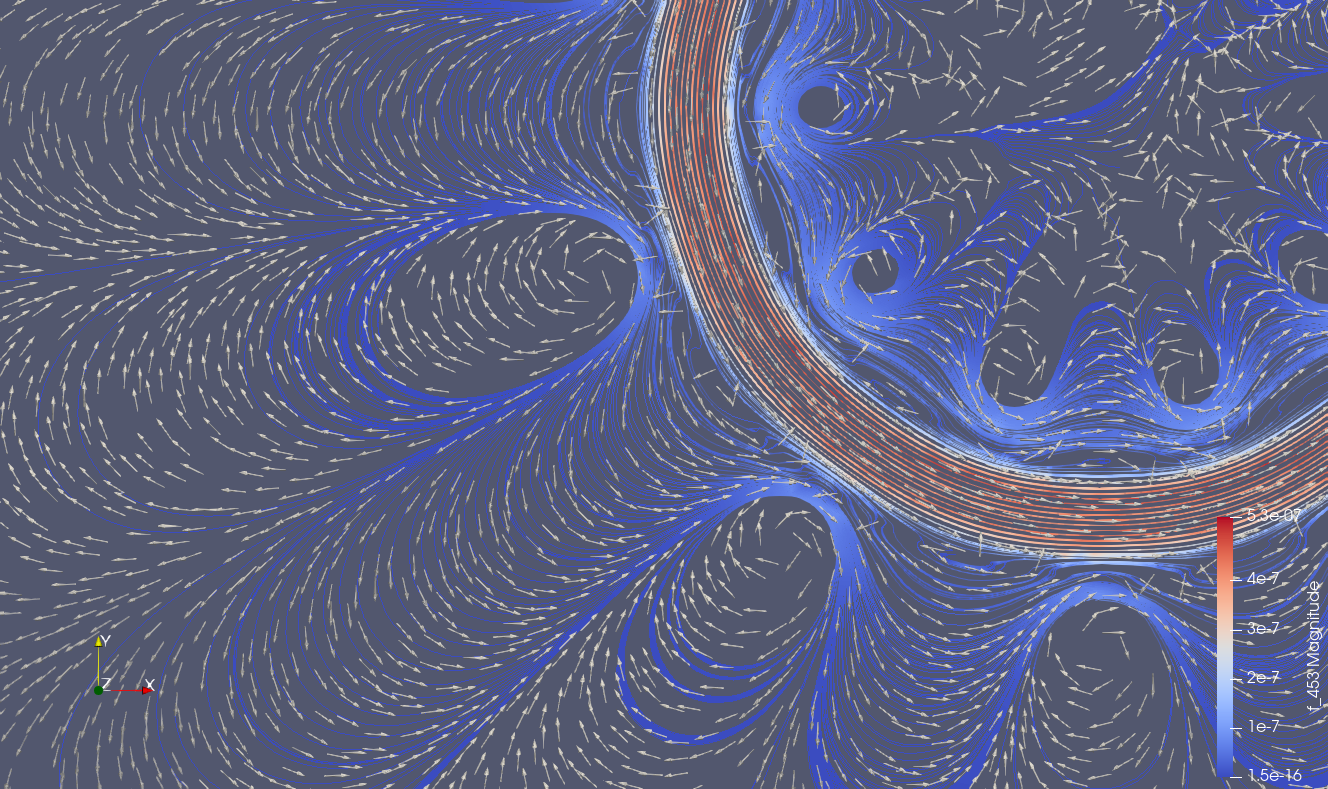
\includegraphics[width=0.45\columnwidth,keepaspectratio]{fenics/test/fenics_electrostatic_case.png}
}\hfill
\subcaptionbox{环形线圈产生的磁场分布示意图}{%
    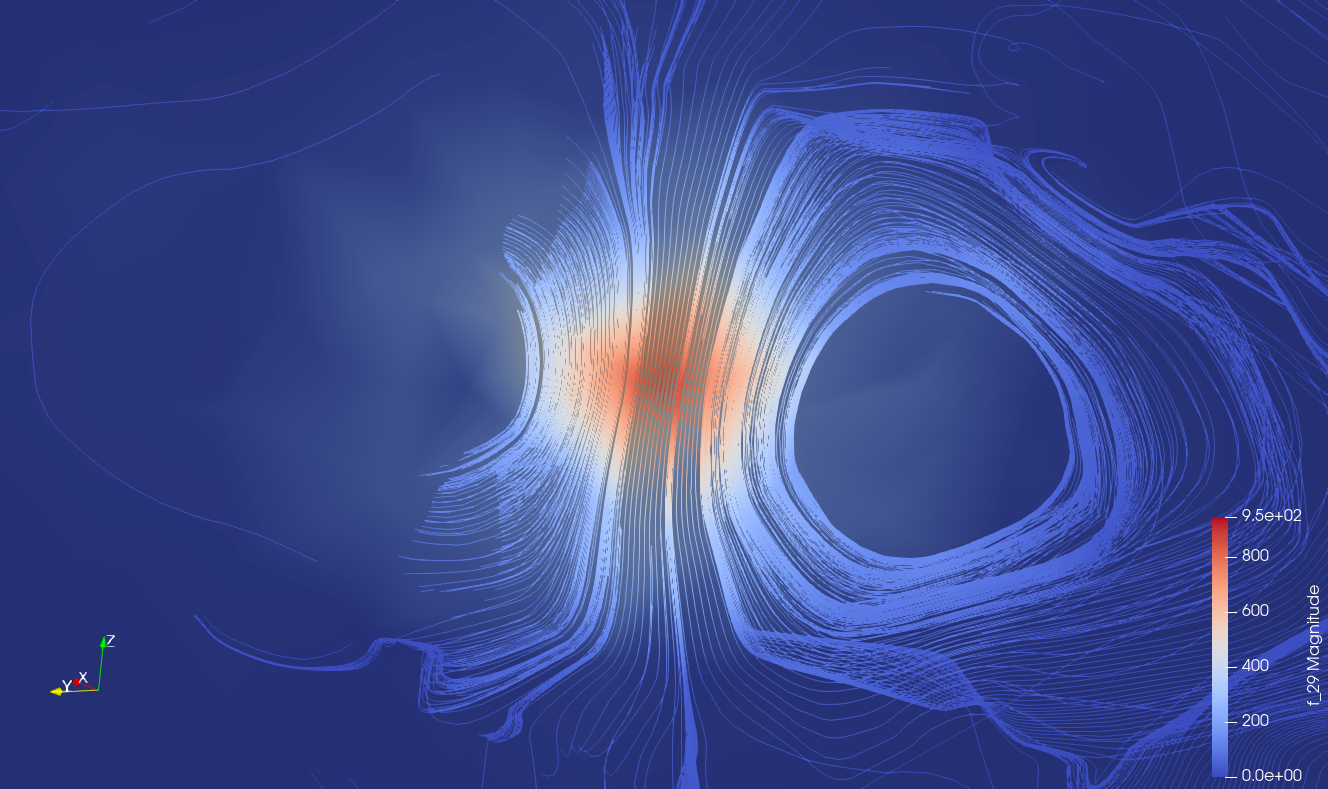
\includegraphics[width=0.45\columnwidth,keepaspectratio]{fenics/test/fenics_coil_B.png}
}%
\label{fig:highm-pos}
\caption{基于 FEniCS 进行的模拟结果}
\end{figure}

